\documentclass{article}

\usepackage{mathrsfs,amsmath}
\usepackage{xcolor}
\usepackage{titlesec}
\usepackage{listings}
\usepackage{syntax}
\usepackage{pythonhighlighting}
\usepackage{graphicx}

\graphicspath{ {./assets/} }

\usepackage[margin=1.4in]{geometry}

\title{Handouts \#1 | CS 471} 
\author{Jared Dyreson\\ 
        California State University, Fullerton}

\usepackage [english]{babel}
\usepackage [autostyle, english = american]{csquotes}
\MakeOuterQuote{"}

\titlespacing*{\section}
{0pt}{5.5ex plus 1ex minus .2ex}{4.3ex plus .2ex}
\titlespacing*{\subsection}
{0pt}{5.5ex plus 1ex minus .2ex}{4.3ex plus .2ex}

\usepackage{hyperref}
\hypersetup{
    colorlinks,
    citecolor=black,
    filecolor=black,
    linkcolor=black,
    urlcolor=black
}

\begin{document}

\maketitle
\tableofcontents

\newpage

\section{Questions}

\textbf{Note: } The Quizlet for this class can be found \href{https://quizlet.com/480232264/471-1-6-flash-cards/}{\underline{here}} and can be referenced instead of this and subsequent documents.

\begin{enumerate}

\item What is a network edge?
\begin{itemize}
\item The area in which a device or local network interfaces with the Internet.
\end{itemize}


\item What is the network core?
\begin{itemize}
\item The infrastructure that connects together the different networks that make up your computer system
\item Mesh of interconnected routers.
\end{itemize}


\item What is a protocol?
\begin{itemize}
\item A means of communication between tow or or more computers given a specific format, the order in which the messages are sent/received and action take once transmitted.
\end{itemize}

\item What is the difference between circuit and packet switching? What are the advantages and disadvantages of each?
\begin{itemize}
\item \href{https://byjus.com/physics/difference-between-circuit-switching-and-packet-switching/}{Advantages/Disadvantages are found \underline{here}}
\item Circuit Switching: establishing a dedicated communication path between the sender and the receiver.
\item Packet Switching: connectionless network where the messages are divided and grouped together (packet).
\end{itemize}

\item What is store and forward architecture? Why is it necessary?
\begin{itemize}
\item Store-and-forward: a message sent by the source device and saved onto an intermediary device (server). This can then be relayed to the final destination and is used when the source device cannot directly communicate with the destination. Think redstone repeater.
\end{itemize}

\item Who long does it take to transmit 1000 bit packet across a 20 bps link?
\begin{itemize}
\item $\frac{1000 \text{ bits }}{20 \text{ bits per second }} \implies 50 \text{ seconds}$
\end{itemize}

\item How long does it take to transmit a 1000 bit packet from system A to system be if:
\begin{itemize}
\item A and B are connected through a router
\item A is connected to the router a 10 bps link
\item B is connected to the router through a 20 bps link
\item Solution: $\frac{1000}{10} + \frac{1000}{20} = 100 + 50 = 150$. Each packet must pass through each link from system to router.
\end{itemize}

\newpage
\item What is the difference between frequency division multiplexing and time division multiplexing? What are the advantages of each?
\begin{itemize}
\item Frequency division multiplexing: sending two or more signals over the same channel where each signal is transmitted as a unique range of frequencies within the bandwidth of the channel as a whole.
\item Time division multiplexing: each signal is sent as a series of packets/pulses, which are interleaved with those of other signals transmitted as a continuous stream. Also, time on the cable is broken up into time slots, each user gets a dedicated time slot.
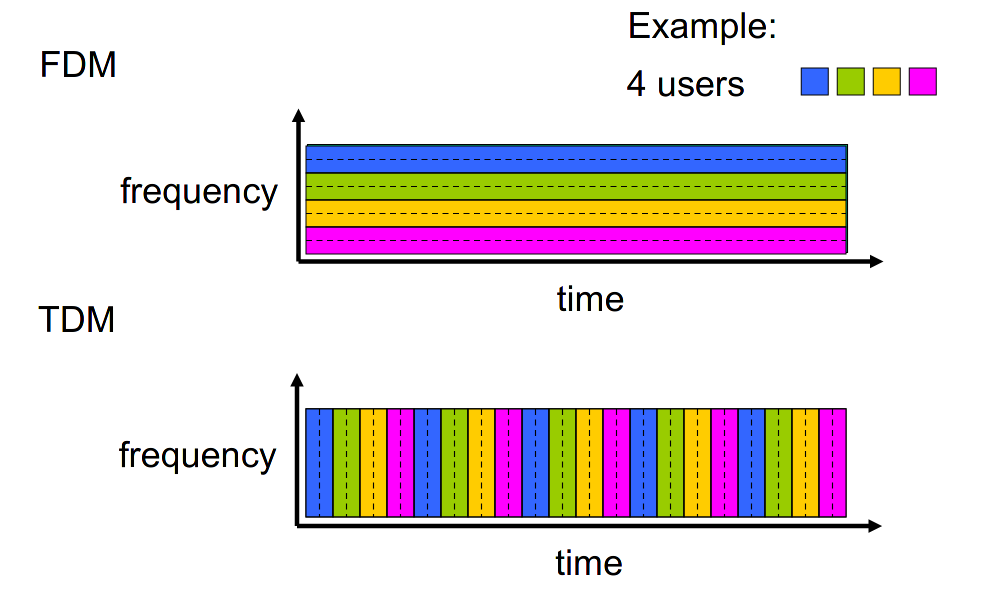
\includegraphics[width=10cm]{FDM_TDM}
\end{itemize}

\end{enumerate}

\end{document}

